\section{Minimum lokalne i globalne}

\subsection{Wprowadzenie}

  \begin{frame}{Wprowadzenie}
    Predstawione powyżej metody działają przy założeniu:\\
    $F(x)$ -- \emph{unimodalna} (w badanym obszarze)
    \begin{block}{Zwykle $F(x)$ ma wiele minimów $\Rightarrow$ wtedy 4 możliwości:}
      \begin{enumerate}
        \item \emph{wystarca znajomość dowolnego minimum lokalnego}\\
        $\to$ rzadko; najprościej
        \item \emph{szukamy minimum globalnego}\\
        $\to$ najczęściej $\Rightarrow$ zwłaszcza w optymalizacji;\\
        brak ogólnych pewnych metod % TODO: underline "pewnych"

      \end{enumerate}
    \end{block}
  \end{frame}

  \begin{frame}{Wprowadzenie}
    \begin{block}{}
      \begin{enumerate}
        \setcounter{enumi}{2}
        \item \emph{interesuje nas jedno ("fizyczne") minimum
        (niekoniecznie) globalne}\\
        $\to$ w badaniach naukowych; z góry znana przybliżona
        lokalizacja minimum $\to$ "dobra dolina". \\
        Poszukiwanie: od ustalenia przybliżonych, przewidywanych
        wartości części parametrów, znalezienie minimum ze
        względu na wszyskie parametry.
        \item \emph{szukamy wszyskich lokalnych minimów
        (w tym globalnego)} \\
        $\to$ najtrudniej, brak ogólnej metody
      \end{enumerate}
    \end{block}
  \end{frame}

\subsection{Algorytm Gelfanda-Cetlina (stepping m.)}
  \begin{frame}{Algorytm Gelfanda-Cetlina (stepping m.)}
    \begin{center}
      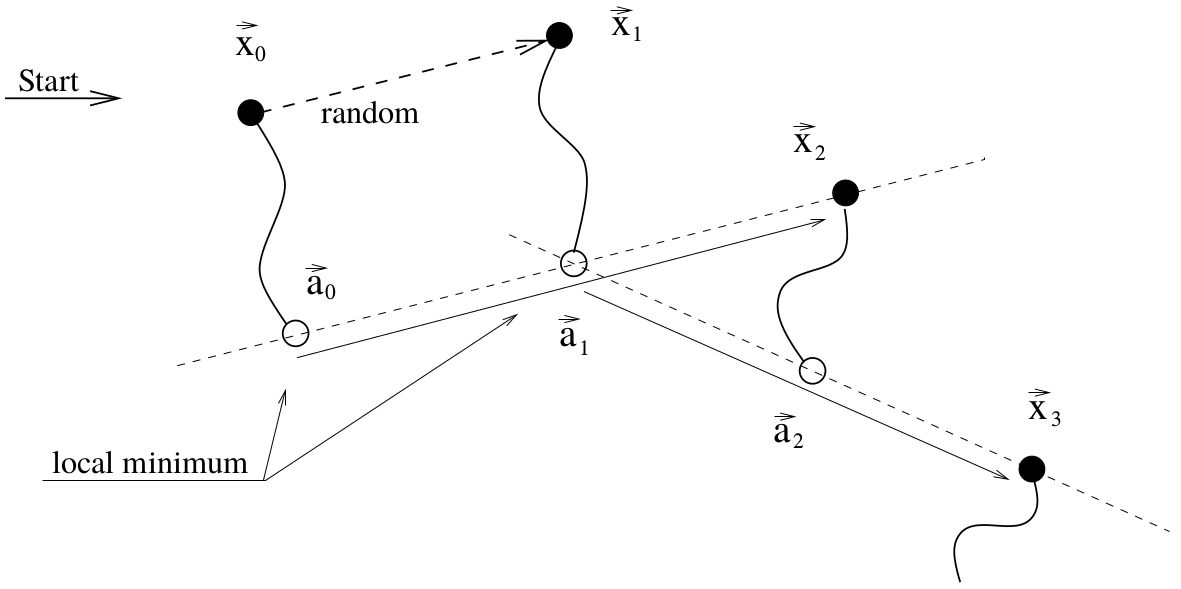
\includegraphics[width=1\textwidth]{img/17/algo_g-c}
    \end{center}
  \end{frame}

  \begin{frame}{Algorytm Gelfanda-Cetlina (stepping m.)}
    \begin{enumerate}
      \item z $\vec{x_{0}}$ -- lokalna minimalizacja $\Rightarrow$
      min. w $\vec{a_{0}}$
      \item z $\vec{x_{0}}$ -- długi, losowy krok do $\vec{x_{1}}$
      \item z $\vec{x_{1}}$ -- lokalna minimalizacja $\Rightarrow$
      min. w $\vec{a_{1}}$
      \item długi krok (precipitous step) wzdłuż
      $\vec{a_{1}} - \vec{a_{0}}$ do $\vec{x_{2}}$
      \item z $\vec{x_{2}}$ -- lokalna minimalizacja $\Rightarrow$
      min. w $\vec{a_{2}}$
      \item długi krok wzdłuż $\vec{a_{2}} - \vec{a_{1}}$ \dots itd.
    \end{enumerate}
  \end{frame}
